\documentclass{standalone}
%outline around text
\usepackage[outline]{contour}
\contourlength{1.3pt}

%tikz
\usepackage{tikz}
\usetikzlibrary{knots, cd, calc}

\begin{document}
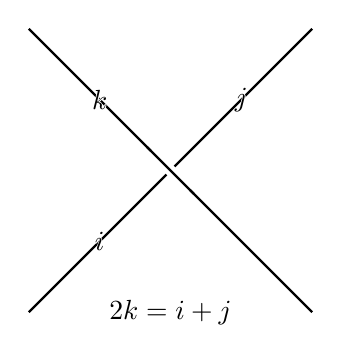
\begin{tikzpicture}[scale=0.9]
\begin{knot}[clip width = 5, flip crossing = 1]
\strand[thick] (-2, -2) -- (2, 2);
\strand[thick] (-2, 2) -- (2, -2);
\end{knot}
\node at (-1, -1) {\contour{white}{$i$}};
\node at (1, 1) {\contour{white}{$j$}};
\node at (-1, 1) {\contour{white}{$k$}};
\node at (0, -2) {$2k = i + j$};
\end{tikzpicture}
\end{document}